\section{Questão 1}
Escolhemos o seguinte sistema:
\begin{equation}
\ddot{x} = (1-e^{-x^2})(x-1)(x-2)
\end{equation}
Cuja descrição em variáveis de estado é:
\begin{equation}
x_1 = x
\end{equation}
\begin{equation}
x_2 = \dot{x}
\end{equation}
\begin{equation}
\dot{x_1} = x_2
\end{equation}
\begin{equation}
\dot{x_2} = (1-e^{-x_1^2})(x_1-1)(x_1-2)
\end{equation}

Cujos pontos de equilíbrio são:
\begin{equation}
[0~0]^T; [1~0]^T; [2~0]^T
\end{equation}

O ponto $[2~0]^T$ é instável, pois para qualquer x(0) escolhido em sua vizinhança a tendência da trajetória é de se afastar do ponto para $t\rightarrow\infty$.\\

O ponto $[1~0]^T$ é estável, pois para x(0) escolhido numa vizinhança suficientemente próxima dele, a tendência da trajetória é de se manter dentro daquela vizinhança $\forall t$.\\

O ponto $[0~0]^T$ é um foco instável, pois para x(0) escolhido numa vizinhança arbitrariamente próxima dele, a tendência da trajetória é de se aproximar da vizinhança do ponto $[1~0]^T$.

\begin{figure}
\includegraphics[width = 14 cm, height = 6 cm]{PlanoDeFaseQ1V0}
\caption{Mapa de Fase, x(0) na vizinhança de $[0~0]^T$}
\end{figure}
\begin{figure}
\includegraphics[width = 14 cm, height = 6 cm]{PlanoDeFaseQ1V1}
\caption{Mapa de Fase, x(0) na vizinhança de $[1~0]^T$}
\end{figure}
\begin{figure}
\includegraphics[width = 14 cm, height = 6 cm]{PlanoDeFaseQ1V2}
\caption{Mapa de Fase, x(0) na vizinhança de $[2~0]^T$}
\end{figure}

\section{Questão 2}
Escolhemos um sistema massa-mola sem atrito onde todas as constantes envolvidas são iguais a 1, de forma que:
\begin{equation}
\ddot{x} = -x
\end{equation}
Onde x é o deslocamento da mola, e cuja descrição em variáveis de estado é:

\begin{equation}
x_1 = x
\end{equation}
\begin{equation}
x_2 = \dot{x}
\end{equation}
\begin{equation}
\dot{x_1} = x_2
\end{equation}
\begin{equation}
\dot{x_2} = -x1
\end{equation}

E cujo retrato de fase é uma circunferência em torno do ponto de equilíbrio, indicando que na medida em que a trajetória evolui, a energia se mantém constante, pois se transfere entre as variáveis de estado $x_1$ e $x_2$.

\begin{figure}
\includegraphics[width = 14 cm, height = 6 cm]{PlanoDeFaseQ2}
\caption{Mapa de Fase, $x(0)=[1~0]^T$}
\end{figure}

\section{Questão 3}

\begin{figure}
\includegraphics[width = 14 cm, height = 6 cm]{PlanoDeFaseQ3Dentro}
\caption{Mapa de Fase, $x(0)=[1~-1]^T$}
\end{figure}

\begin{figure}
\includegraphics[width = 14 cm, height = 6 cm]{PlanoDeFaseQ3Fora}
\caption{Mapa de Fase, $x(0)=[1~-3]^T$}
\end{figure}


 Dadas a descrição do sistema por variáveis de estado:
 \begin{equation}
 \dot{x_1} = x_2
 \end{equation}
  \begin{equation}
  \dot{x_2} = -x_1+x_2-x_2^3/3
  \end{equation}
 Se temos $\dot{x}=0$ isto implica que $x_2=0$ e $x_1=0$, a origem é o único ponto de equilíbrio do sistema. Pelo Teorema de Poincaré temos N-S=1, ou seja, pode existir um ciclo limite.\\
 
 Pelo Teorema de Poincaré-Bendixson, e fazendo a conversão para coordenadas polares, temos:\\
 
 \begin{equation}
 r = \sqrt{x_1^2 + x_2^2}
 \end{equation} 
\begin{equation}
\dot{r} = \frac{1}{\sqrt{x_1^2+x_2^2}}(x_1\dot{x_1} + x_2\dot{x_2})
\end{equation}

\noindent Que resulta em:

\begin{equation}
\dot{r} = \frac{1}{r}(r^2\sin^2\theta-r^4\sin^4\theta)
\end{equation}

\noindent De forma que para $r=\frac{\sqrt{3}}{\sin\theta}$ temos que $\dot{r}$ muda de sinal. Enquanto $r<\frac{\sqrt{3}}{\sin\theta}$,$\dot{r}>0$ e para  $r>\frac{\sqrt{3}}{\sin\theta}$,$\dot{r}<0$: existe um região anular para a qual a trajetória tende a convergir. Existe ciclo limite. 

Pelo teorema de Bendixson, analisando o traço do Jacobiano:

\begin{equation}
1-x_2^2=0
\end{equation}

Implica que para $|x_2|>1$ o traço muda de sinal. Como o traço não muda de sinal para $|x_2|<1$, o ciclo limite existe e sua amplitude em relação a $x_2$ deve ser maior que 1.

\section{Questão 4}
Para o sistema descrito em variáveis de estado por:
\begin{equation}
\dot{x_1} = x_2
\end{equation}
\begin{equation}
\dot{x_2} = -\sigma x_1
\end{equation}
\begin{equation}
\sigma = sign(x_1(x_1+cx_2))
\end{equation}

\noindent O mapa de fase pode ser desenhado através da reta auxiliar $x_2 = -x_1/c$, que indica as mudanças de sinal de $\sigma$. Para $x_1>0$ e $x_2<-x_1/c$ temos $\sigma=-1$. Para $x_1<0$ e $x_2>-x_1/c$ temos $\sigma=-1$. Em todas as outras condições $\sigma=1$. Desta forma, uma trajetória qualquer seguirá o padrão de um sistema conservativo até que entre numa região onde $\sigma$ assume sinal negativo. Quando isto acontecer a inclinação da trajetória irá ser "rebatida", de forma que, se por exemplo, a inclinação antes de entrar na região era de $26,6^o$ (c=0.5), após entrar na região será de $-26,6^o$.\\ 

É interessante notar que para c>1 a tendência da trajetória após entrar na região onde $\sigma=-1$ é de sair desta mesma região. Isto indica que o sistema irá chavear com frequência infinita levando a trajetória até a origem. Confirmamos este comportamento para c um pouco maior que 1 nas simulações, assim como para c=2.\\
\begin{figure}
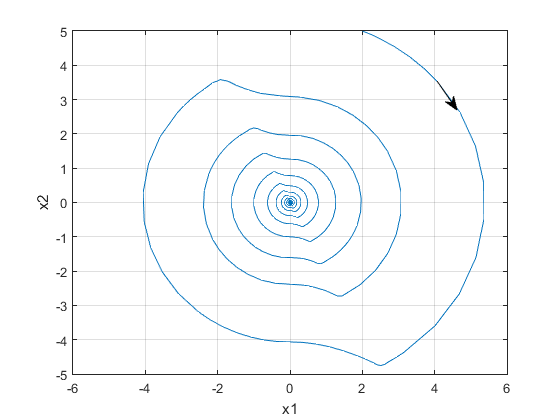
\includegraphics[width = 14 cm, height = 6 cm]{PlanoDeFaseQ4C05P1}
\caption{Mapa de Fase, x(0)=$[2~5]^T$, c=0.5}
\end{figure}
\begin{figure}
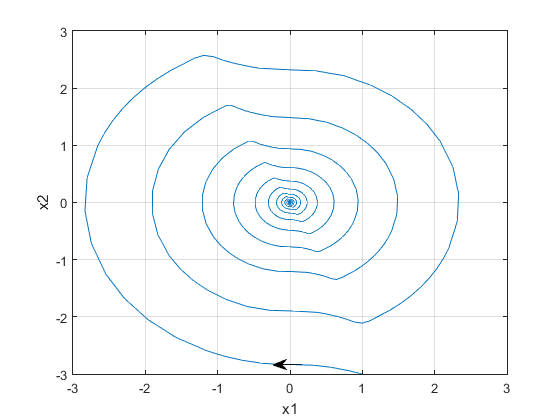
\includegraphics[width = 14 cm, height = 6 cm]{PlanoDeFaseQ4C05P2}
\caption{Mapa de Fase, x(0)=$[1~-3]^T$, c=0.5}
\end{figure}
\begin{figure}
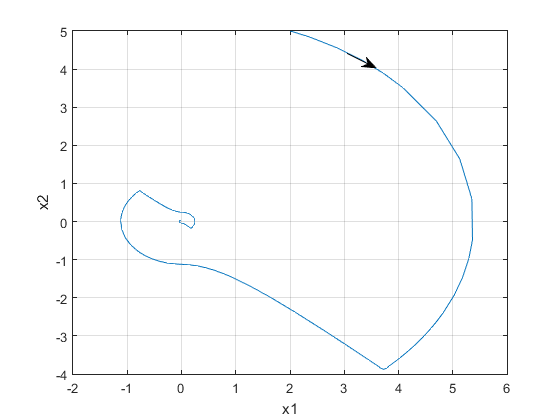
\includegraphics[width = 14 cm, height = 6 cm]{PlanoDeFaseQ4C10P1}
\caption{Mapa de Fase, x(0)=$[2~5]^T$, c=1}
\end{figure}
\begin{figure}
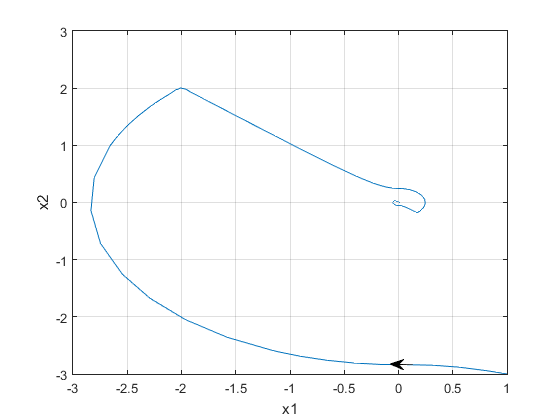
\includegraphics[width = 14 cm, height = 6 cm]{PlanoDeFaseQ4C10P2}
\caption{Mapa de Fase, x(0)=$[1~-3]^T$, c=1}
\end{figure}
\begin{figure}
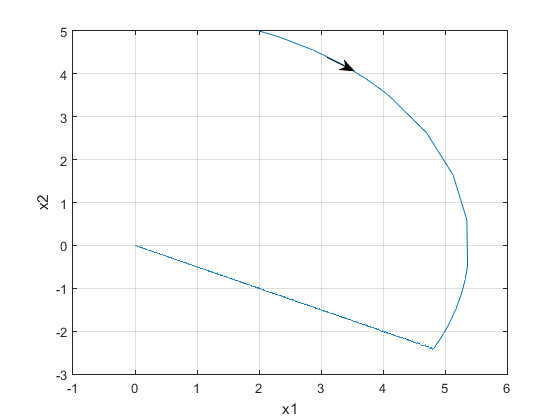
\includegraphics[width = 14 cm, height = 6 cm]{PlanoDeFaseQ4C20P1}
\caption{Mapa de Fase, x(0)=$[2~5]^T$, c=2}
\end{figure}
\begin{figure}
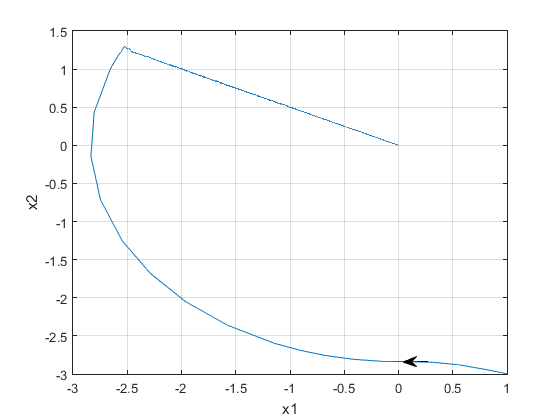
\includegraphics[width = 14 cm, height = 6 cm]{PlanoDeFaseQ4C20P2}
\caption{Mapa de Fase, x(0)=$[1~-3]^T$, c=2}
\end{figure}
\begin{figure}
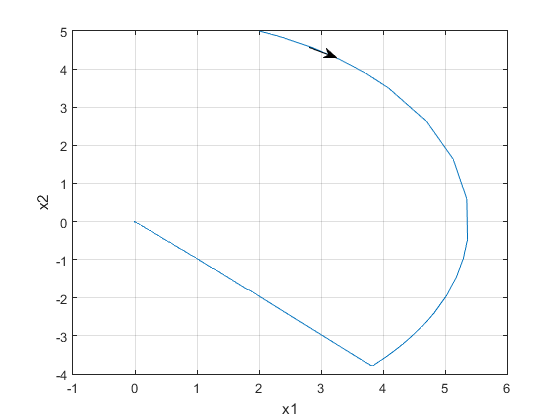
\includegraphics[width = 14 cm, height = 6 cm]{PlanoDeFaseQ4C103P1}
\caption{Mapa de Fase, x(0)=$[2~5]^T$, c=1.03}
\end{figure}
\begin{figure}
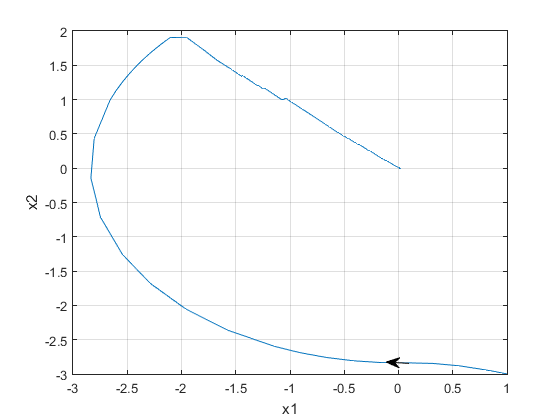
\includegraphics[width = 14 cm, height = 6 cm]{PlanoDeFaseQ4C108P2}
\caption{Mapa de Fase, x(0)=$[1~-3]^T$, c=1.08}
\end{figure}

\section{Questão 5}

a) Para o relé puro temos que $N(X) = \frac{4M}{\pi X}$. Para $G(jw)$ tal que $Im(G(jw))=0$ temos $G(jw)= \frac{K}{jw(1+jwT)(1+jwaT)}$, precisamos que $1-w^2aT^2=0$, que implica em $w=\frac{1}{\sqrt{a}T}$. Que leva a $x(t)=X\sin wt = \frac{4MKaT\sin(t/(\sqrt{a}T))}{\pi(1+a)}$. Como o cálculo feito foi literal e temos a garantia de que a>0, T>0 e K>0, sempre existirá ciclo limite.\\

b) Da letra a) temos $w=\frac{1}{\sqrt{a}T}$ e a amplitude $X=\frac{4MKaT}{\pi(1+a)}$.\\

c) Para $X<\frac{4MKaT}{\pi(1+a)}$ temos $G(jw)$ passando à esquerda do ponto -1/N(X) no eixo real, o que indica que a amplitude aumenta. Para $X>\frac{4MKaT}{\pi(1+a)}$ temos $G(jw)$ passando à direita do ponto -1/N(X) no eixo real, o que indica que a amplitude diminui. O ciclo limite é estável.\\

d)Alta frequência de oscilação e baixa amplitude.\\

e)Para K=M=T=1 e a=0.1 temos w=3.1623 para que $G(jw)$ intercepte o eixo real. Para que não haja ciclo limite, é necessário que a zona morta do relé invalide a equação $X=-GNX$, de forma que $-G(jw)N(X)\neq1$. O valor de $G(jw)$ que intercepta o eixo real é 0.1/1.1, caso a zona morta seja maior que este valor, não poderá haver ciclo limite.\\

f)Nas condições de e) basta calcular a atenuação para a segunda harmônica, caso o valor seja alto o suficiente a hipótese do filtro se mantém. Para w=6.3246 temos uma atenuação da ordem de $1/246 \approx 0.004$, a atenuação para a primeira harmônica é de aproximadamente 0.09, de forma que a primeira harmônica é atenuada aproximadamente 22 vezes menos que a segunda harmônica (~16dB). A hipótese do filtro se mantém.